\documentclass{article}
\usepackage[utf8]{inputenc}
\usepackage[czech]{babel}
\usepackage[T1]{fontenc}% umožňuje kopírovat znaky z výstupu
\usepackage{amsmath}
\usepackage{amsfonts}
\usepackage{amssymb}
\usepackage{enumitem}% číslované odrážky

\usepackage{graphicx}

\graphicspath{ {./images/} }
\graphicspath{ {./figures/} }
\usepackage{svg}

\usepackage{hhline}

\usepackage{listings}
\usepackage{xcolor}

\usepackage{siunitx}% desetnná tečka
\usepackage{makecell}

\usepackage{multirow}

\usepackage{pdfpages}%pro přidání celé stránky pdf

\usepackage{booktabs}%zarovnání \toprule, \midrule a \bottomrule
\usepackage{blindtext}% generování náhodného textu \blindtext
\usepackage{hyperref}%přídání klikatelné reference \href{https://www.example.com}{Example}
\usepackage{geometry}%nastavení okrajů pro text
\geometry{left=25.4mm, right=25.4mm, top=25.4mm, bottom=25.4mm}%okraje jako ve wordu
\usepackage{setspace}
\setlength{\parindent}{1cm} % nastaví odsazení odstavců na 1 cm
\usepackage{float}
\restylefloat{table}
\normalsize

\title{Dokumentace}
\author{}
\date{\vspace{-1.0cm}}% defaultně tady bývá datum... posunul jsem o jeden cm výš
\newcommand{\mysubsection}[1]{\hspace{1 cm}\subsection*{#1}\setstretch{1.5}}

\begin{document}


\includepdf[pages=-]{rozpiska.pdf}

\maketitle

\subsection*{Úvod:}
\setstretch{1.2}%řádkování
\hspace{1 cm}
Jako téma projektu z informatiky byla zvolena tvorba mobilní aplikace pro export dat z Arduina. Cílem bylo vytvořit mobilní aplikaci, která by umožnila export dat z Arduina do mobilního zařízení prostřednictvím Bluetooth. Toto téma bylo zvoleno, jelikož Arduino neumí samo o sobě ukládat data a pokud jsou data ukládána na SD kartu, v okamžiku, kdy potřebujeme data získat, je nutné SD kartu vyjmout. To vede k problému, že během stahování dat nelze ukládat nově generovaná data. Cílem naší aplikace je vyřešit tento problém tím, že data budou ukládána na SD kartu a v případě potřeby exportu dat budou exportována prostřednictvím Bluetooth do námi vytvořené mobilní aplikace.

\subsection*{Návrh aplikace:}
\input{tex/02_Návrh_aplikace}

\subsection*{Návod spuštění kódu aplikace:}
\setstretch{1.2}%řádkování
\hspace{1 cm}
Pro kopii: \texttt{git clone \href{https://github.com/kovarmi9/PJIN\_mobilni\_bluetooth\_aplikace}{https://github.com/kovarmi9/PJIN\_mobilni\_bluetooth\_aplikace}.git}.
Pro spuštění kódu aplikace je potřeba mít nainstalovaný \textbf{Node.js} a \textbf{npm}. \textbf{Node.js} je prostředí, které umožňuje spouštění \textbf{JavaScriptu(TypeScriptu)} mimo prohlížeč. \textbf{Npm (Node Package Manager)} je balíčkovací systém pro \textbf{JavaScript}, který je součástí instalace \textbf{Node.js}. \textbf{Node.js} a \textbf{npm} lze stáhnout ze stránek:\href{https://nodejs.org/en}{https://nodejs.org/en}. Dále bude potřeba \textbf{React Native CLI}. \textbf{React Native CLI} je nástroj, který umožňuje vytvářet a spravovat projekty \textbf{React Native}. Lze jej nainstalovat pomocí \textbf{npm} příkazem \texttt{npm install -g react-native-cli}. 
Po instalaci těchto nástrojů je potřeba ještě zařízení na němž bude probíhat ladění kódu aplikace. K tomu může posloužit virtuální zařízení. Virtuální zařízení \textbf{Android} zle vytvořit s pomocí \textbf{Android Studia} nebo pro tvorbu virtuálního zařízení s \textbf{iOS} bude potřeba \textbf{Mac} a software \textbf{Xcode}. Virtuální zařízení ovšem nepodporují práci s Bluetooth a tak je lepší alternativou pro ladění aplikace využít skutečné mobilní zařízení s Androidem. Nejprve je nutné na mobilním zařízení povolit možnosti pro vývojáře. To se provede v \texttt{nastavení} \(\rightarrow\) \texttt{o telefonu} \(\rightarrow\) \texttt{informace o software} \(\rightarrow\) \texttt{číslo sestavení} a po té co je sedmkrát poklepáno na možnost \texttt{číslo sestavení} se otevřou možnosti pro vývojáře. Dále je nutné v možnostech pro vývojáře povolit možnost \texttt{Ladění USB}. Po té co je toto nastavení provedeno, je mobilní zařízení připojeno k počítači prostřednictvím USB kabelu a je v adresáři s projektem v terminálu spuštěn příkaz \texttt{npm start} a zvolena možnost \texttt{a} pro Android se na mobilním zařízení vytvoří prostředí aplikace, které se přizpůsobuje změnám kódu. Před prvním spuštěním aplikace je ještě potřeba do terminálu v adresáři s projektem zadat příkaz \texttt{npm install} který by měl automaticky nainstalovat všechny balíčky, které jsou využívány v projektu.

\subsection*{Návod instalace:}
\setstretch{1.2}%řádkování
\hspace{1 cm}
Aplikaci lze nainstalovat s pomocí instalačního souboru, který lze stáhnout do mobilního zařízení z adresáře: \href{https://github.com/kovarmi9/PJIN_mobilni_bluetooth_aplikace/blob/main/instalacni_soubor.apk}{https://github.com/kovarmi9/PJIN\_mobilni\_bluetooth\_aplikace/blob/main/instalacni\_soubor.apk} po kliknutí na „View raw“.

\begin{figure}[H]
    \centering
    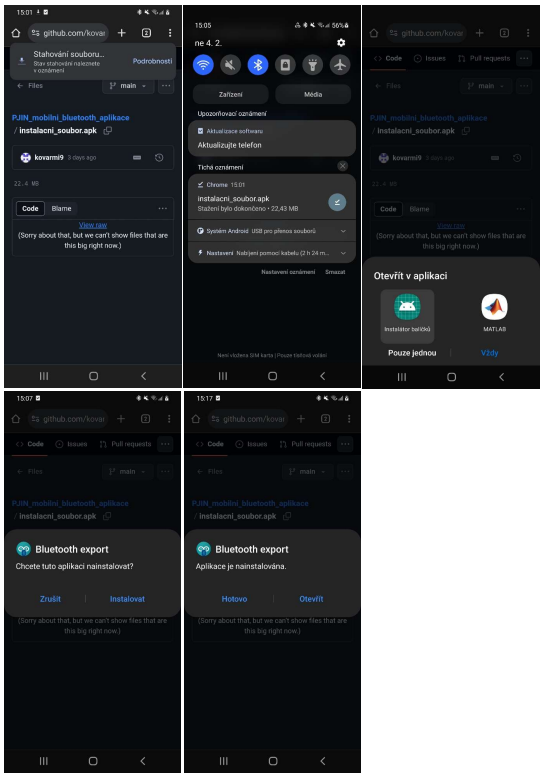
\includegraphics[width=0.5\textwidth]{images/navod_instalace.png}
    \caption{Návod instalace aplikace s pomocí instalačního souboru}
\end{figure}


\subsection*{Návod používání aplikace:}
\setstretch{1.2}%řádkování
\hspace{1 cm}
Po spuštění aplikace se otevře dotazové okno, kde je nutné povolit přístup k poloze zařízení (z důvodu že knihovna pro práci s Bluetooth vyžaduje přístup k poloze). Následně se otevře samotná aplikace. Základní grafické rozhraní obsahuje název a stručný popis aplikace, odkaz na GitHub se zdrojovým kódem aplikace a dvě tlačítka - \textbf{1.} připojení zařízení přes Bluetooth, které po rozkliknutí otevře nastavení Bluetooth a zobrazí okolní zařízení, ke kterým se lze připojit, po připojení aplikace zobrazuje název připojeného zařízení; \textbf{2.} export souborů z SD karty zařízení (Arduina), po rozkliknutí tlačítka exportu se zobrazí řádky s názvy souborů uložených na SD kartě připojeného zařízení a k nim přilehlá 3 tlačítka - náhled, stažení a sdílení souboru. Vzhledem k tomu, že se nepodařilo vyřešit problémy s připojováním k Bluetooth zařízení v aplikaci, tak slouží aplikace nainstalovaná pomocí instalačního souboru jako pouhé demo. Na aplikaci je v plánu dále pracovat a další změny budou dostupní na GitHubu.

\begin{figure}[H]
    \centering
    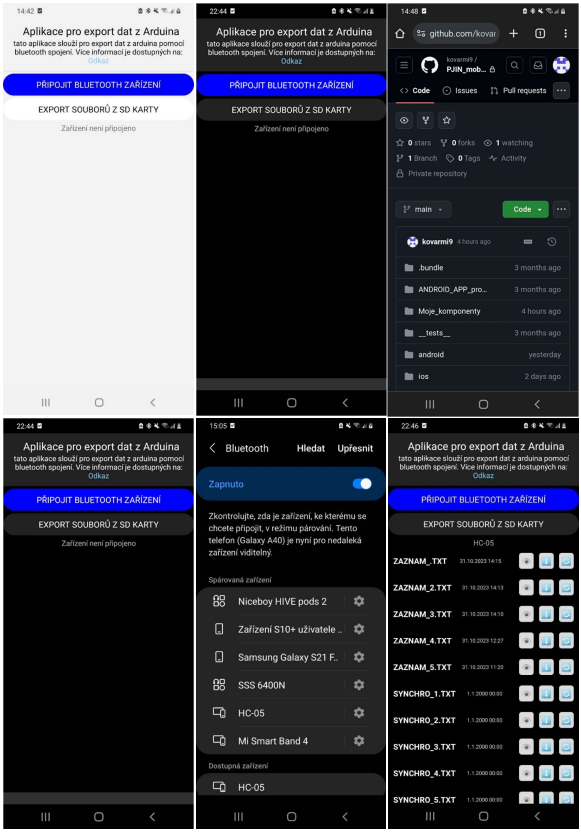
\includegraphics[width=0.5\textwidth]{images/navod_pouzivani.png}
    \caption{Ukázka aplikace}
\end{figure}

\subsection*{Přílohy:}
\setstretch{1.2}%řádkování
\hspace{1 cm}
\begin{tabular}{lll} 
\setstretch{1.2}%řádkování
\hspace{0 cm}\text{Příloha 1} & Github repozitář &  \text{\href{https://github.com/kovarmi9/PJIN_mobilni_bluetooth_aplikace}{https://github.com/kovarmi9/PJIN\_mobilni\_bluetooth\_aplikace}}\\
\end{tabular}

\subsection*{Závěr a zhodnocení:}
\setstretch{1.2}%řádkování
\hspace{1 cm}
Mobilní aplikace má plně vyhotovené grafické uživatelské rozhraní. Plně hotový je také kód pro Arduino. Aplikace je schopná spustit vyhledávání přes Bluetooth a skutečně nalézt blízká zařízení. Aplikace má zatím neodhalený problém v komunikaci s Bluetooth zařízením. Na aplikaci je v plánu dále pracovat, aby byla plně funkční a další změny v aplikaci budou dostupné na GitHubu.


\subsection*{Reference:}
\begin{flushleft}
\label{dratek}[1] Arduino Bluetooth modul HC-05. Návody Drátek. Dostupné z: \url{https://navody.dratek.cz/navody-k-produktum/arduino-bluetooth-modul-hc-05.html}
\end{flushleft}

\begin{flushleft}
\label{arduinoSD}[2] SD - Arduino Reference. Arduino. Dostupné z: \url{https://www.arduino.cc/reference/en/libraries/sd/}
\end{flushleft}

\begin{flushleft}
\label{nodejs}[3] Node.js. Node.js\textsuperscript{\textregistered} is an open-source, cross-platform JavaScript runtime environment. Dostupné z: \url{https://nodejs.org/en}
\end{flushleft}

\begin{flushleft}
\label{reactnative}[4] React Native. Learn once, write anywhere. Dostupné z: \url{https://reactnative.dev/}
\end{flushleft}




\vspace{5 cm}

\noindent
v Praze \today \hfill Michal Kovář a Kryštof Sedlák

\end{document}

